\documentclass{ximera}
\input{../preamble}
\addPrintStyle{..}
\begin{document}
	\author{Wiskunde Op Maat}
	\xmtitle{Kwadratische vergelijkingen oplossen in de complexe getallen}{}


\newcommand{\choicetweer}{{\wordChoice{\choice[correct]{twee reële oplossingen}\choice{een dubbele reële oplossing}\choice{twee complexe oplossingen}}}}
\newcommand{\choicdubbel}{{\wordChoice{\choice{twee reële oplossingen}\choice[correct]{een dubbele reële oplossing}\choice{twee complexe oplossingen}}}}
\newcommand{\choicetweec}{{\wordChoice{\choice{twee reële oplossingen}\choice{een dubbele reële oplossing}\choice[correct]{twee complexe oplossingen}}}}

\newcommand{\choicepositief}{{\wordChoice{\choice[correct]{positief}\choice{nul}\choice{negatief}}}}
\newcommand{\choicenul}{{\wordChoice{\choice{positief}\choice[correct]{nul}\choice{negatief}}}}
\newcommand{\choicenegatief}{{\wordChoice{\choice{positief}\choice{nul}\choice[correct]{negatief}}}}


\begin{exercise}
    Bepaal de oplossingen van de vierkantsvergelijking \(x^2 - 4x + 5 = 0\).  
    
    \begin{question}
    De discriminant is \choicenegatief.
    
    \begin{feedback}
    Het algemene voorschrift van een tweedegraadsvergelijking wordt gegeven door \(ax^2 + bx + c = 0\).
    Om een tweedegraadsvergelijking op te lossen bereken je eerst de discriminant \(\Delta = b^2 - 4ac\).
    \textbf{In de complexe getallen zijn er altijd oplossingen.}
    \end{feedback}
    \end{question}
    
    \begin{question}
    Deze tweedegraadsvergelijking heeft \choicetweec 
    
    \begin{feedback}
    Indien de discriminant \(\Delta = b^2 - 4ac\) negatief is, zijn er twee complexe oplossingen. Waar je in de reële getallen niet verder kon rekenen bij een negatieve discriminant onder de vierkantswortel, vormt dat in de complexe getallen geen probleem. 
    \end{feedback}
    \end{question}
    
    \begin{question}
    Bepaal de wortels.
    
    \begin{hint}
    Voor een tweedegraadsvergelijking \(ax^2 - bx + c = 0\) kan je \textbf{altijd} twee oplossingen te vinden: 
    \[ x_{1,2} = \frac{-b \pm \sqrt{\Delta}}{2a} \]
    met \(\sqrt{\Delta}\) een complex getal.
    \end{hint}
    \end{question}
    
    \begin{oplossing}
    De tweedegraadsvergelijking \(x^2 - 4x + 5 = 0\) heeft de coëfficiënten \(a = 1, b = -4, c = 5\).
    
    De discriminant \( \Delta = (-4)^2 - 4(1)(5) = 16 - 20 = -4 \).
    Aangezien de discriminant negatief is, zijn de wortels complex:
    \[ x_{1,2} = \frac{-(-4) \pm \sqrt{-4}}{2\cdot1} \]
    \[ x_{1,2} = \frac{4 \pm 2i}{2} \]
    \[ x_{1} = 2 + i, \quad x_{2} = 2 - i \]
    
    Dit betekent dat de vergelijking geen reële oplossingen heeft, maar wel twee complexe oplossingen.
    \end{oplossing}
        
\end{exercise}
        


\begin{exercise}
    Bepaal de oplossingen van de vierkantsvergelijking \(2x^2 + 4x + 5 = 0\).  
    
    \begin{question}
    De discriminant is \choicenegatief.
    
    \begin{feedback}
    Het algemene voorschrift van een tweedegraadsvergelijking wordt gegeven door \(ax^2 + bx + c = 0\).
    Om een tweedegraadsvergelijking op te lossen bereken je eerst de discriminant \(\Delta = b^2 - 4ac\).
    \textbf{In de complexe getallen zijn er altijd oplossingen.}
    \end{feedback}
    \end{question}
    
    \begin{question}
    Deze tweedegraadsvergelijking heeft \choicetweec 
    
    \begin{feedback}
    Indien de discriminant \(\Delta = b^2 - 4ac\) negatief is, zijn er twee complexe oplossingen. Waar je in de reële getallen niet verder kon rekenen bij een negatieve discriminant onder de vierkantswortel, vormt dat in de complexe getallen geen probleem. 
    \end{feedback}
    \end{question}
    
    \begin{question}
    Bepaal de wortels.
    
    \begin{hint}
    Voor een tweedegraadsvergelijking \(ax^2 - bx + c = 0\) kan je \textbf{altijd} twee oplossingen te vinden: 
    \[ x_{1,2} = \frac{-b \pm \sqrt{\Delta}}{2a} \]
    met \(\sqrt{\Delta}\) een complex getal.
    \end{hint}
    \end{question}
    
    \begin{oplossing}
    De tweedegraadsvergelijking \(2x^2 + 4x + 5 = 0\) heeft de coëfficiënten \(a = 2, \; b = 4, \; c = 5\).
    
    De discriminant \( \Delta = 4^2 - 4(2)(5) = 16 - 40 = -24 \).
    Aangezien de discriminant negatief is, zijn de wortels complex:
    \[ x_{1,2} = \frac{-4 \pm \sqrt{-24}}{2\cdot2} \]
    \[ x_{1,2} = \frac{-4 \pm 2\sqrt{6}i}{4} \]
    \[ x_{1} = -1 + \frac{\sqrt{6}}{2}i, \quad x_{2} = -1 - \frac{\sqrt{6}}{2}i \]
    
    Dit betekent dat de vergelijking geen reële oplossingen heeft, maar wel twee complexe oplossingen.
    \end{oplossing}
        
\end{exercise}


% twee reele oplossingen 
\begin{exercise}

    Bepaal de oplossingen van de vierkantsvergelijking \(x^2 - 4x + 3 = 0\).   
    
    \begin{question}
    De discrimant is \choicepositief. 
    
    \begin{feedback}
        Het algemene voorschrift van een tweede graadsvergelijking wordt gegeven door  \(ax^2 + bx + c = 0\). 
        Om een tweedegraadsvergelijking op te lossen bereken je eerst de discriminant \(\Delta = b^2 - 4ac\). 
        \textbf{In de complexe getallen zijn er altijd oplossingen.}
        
    \end{feedback}
    \end{question}
    
    \begin{question}
        Deze vergelijking heeft \choicetweer.
        \begin{feedback}
            Indien de discriminant \(\Delta = b^2 - 4ac\) positief is, zijn er twee oplossingen in de reële getallen. Elk reëel getal is ook complex. Je kan het zien als een complex getal mnet imagnair deel \(0i\). In het complexe vlak liggen deze getallen op de reële-as.  
        \end{feedback}
    \end{question}
    
    \begin{question}
        Bepaal de wortels. 
        
        \begin{hint}
            
            Voor een tweedegraadsvergelijking  \(ax^2 - bx + c = 0\) waarbij de discriminant \( \Delta = b^2 - 4ac \) positief is hebben we altijd twee oplossing gegeven door: 
            
            \[
                x_{1} = \frac{-b + \sqrt{\Delta}}{2a}  \text{ en }  x_{2} = \frac{-b - \sqrt{\Delta}}{2a}
                \]
                
                Waarbij:
                \begin{itemize}
                    \item \( a \) de coëfficiënt van \( x^2 \) is,
                    \item \( b \) de coëfficiënt van \( x \) is,
                    \item \( c \) de constante term is,
                \end{itemize}
                
        \end{hint}
        
    
    \end{question}
    
    \begin{oplossing}
                
    In het algemeen wordt een tweedegraadsvergelijking in één onbekende gegeven door het voorschrift \(ax^2 - bx + c = 0\). 
    De tweedegraadsvergelijking \(x^2 - 4x + 3 = 0\) heeft als coëfficiënten gelijk aan \(a = 1, b = -4 \text{ en } c = 3\). 
    We zoeken de getalwaarden voor \(x\) waarvoor deze vergelijking gelijk is aan nul. 
    Hiervoor kan de formule met discrimant gebruikt worden. 
    
    \vspace{5mm}
    
    De discrimant \( \Delta = b^2 - 4ac \) is gelijk aan \(\Delta = (-4)^2 -4\cdot 1 \cdot 3\). De vierkanswortel wordt dan gegeven door \(\sqrt{\Delta} = \sqrt{4} = 2\). Er zijn dus twee oplossingen omdat de discriminant positief is. Deze oplossingen worden gegeven door: 
    
    \[
    x_{1} = \frac{-b + \sqrt{\Delta}}{2a}  \text{ en }  x_{2} = \frac{-b - \sqrt{\Delta}}{2a}
    \]
    
    Invullen levert: 
    
    \[
    x_{1} = \frac{-(-4) + \sqrt{4}}{2\cdot 1}  = 3 
    \]
    
    
    \[
    x_{2} = \frac{-(-4) - \sqrt{4}}{2\cdot 1}  = 1
    \]
     
    
    Als je de vergelijking beschouwt als een functievoorschrift, zijn deze oplossingen de snijpunten van de parabool \( f(x) = x^2 - 4x + 3 \) met de \(x\)-as. Aangezien de discriminant positief is, zal de parabool de \(x\)-as 2 keer snijden. 
    
    \begin{image}
    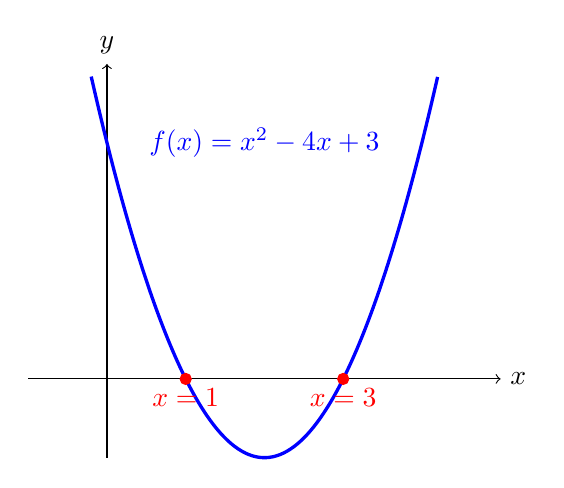
\begin{tikzpicture}[scale=1]
    
        % Draw axes
        \draw[->] (-1,0) -- (5,0) node[right] {\(x\)};
        \draw[->] (0,-1) -- (0,4) node[above] {\(y\)};
        
        % Draw the parabola y = x^2 - 4x + 3
        \draw[domain=-0.2:4.2, samples=100, smooth, very thick, blue] 
            plot (\x, {(\x)^2 - 4*(\x) + 3}); 
            
        \draw (2, 3) node[blue] {\( f(x) = x^2 - 4x + 3 \)};
    
        % Roots (zeros) of the parabola
        \filldraw[red] (1,0) circle (2pt) node[below] {\(x=1\)};
        \filldraw[red] (3,0) circle (2pt) node[below] {\(x=3\)};
    
    \end{tikzpicture}
    \end{image}
    
    Met de discrimantformule bereken je dus deze snijpunten met de \(x\)-as zonder grafiek van de functie . 
    \end{oplossing}
      
        
    \end{exercise}
    
\begin{exercise}
    
    
    \begin{question} \(  x^2 - 6x + 10 = 0   \) \begin{uitkomst} Er zijn twee complexe oplossingen  \(  3 + i                              \) en  \(  3 - i                              \) \end{uitkomst} \end{question}
    \begin{question} \( x^2 + 2x - 8    = 0  \) \begin{uitkomst} Er zijn twee reële oplossingen  \( -4 \) en \( 2 \)           \end{uitkomst} \end{question}
    \begin{question} \(  x^2 + 2x + 2 = 0    \) \begin{uitkomst} Er zijn twee complexe oplossingen  \( -1 + i                              \) en  \( -1 - i                              \) \end{uitkomst} \end{question}
    \begin{question} \( 3x^2 - 6x + 3        \) \begin{uitkomst} De dubbele wortel is gelijk aan    \(  1                                                                                \) \end{uitkomst} \end{question}
    \begin{question} \(  3x^2 - 6x + 7 = 0   \) \begin{uitkomst} Er zijn twee complexe oplossingen  \(  1 + \frac{2i}{\sqrt{3}}            \) en  \(  1 - \frac{2i}{\sqrt{3}}            \) \end{uitkomst} \end{question}
\end{exercise}

\begin{exercise}

    \begin{question} \( x^2 + 4x + 8 = 0     \) \begin{uitkomst} Er zijn twee complexe oplossingen  \( -2 + i                              \) en  \(  -2 - i                             \) \end{uitkomst} \end{question}
    \begin{question} \( 2x^2 + 5x + 2        \) \begin{uitkomst} Er zijn twee reêle oplossingen     \( -\frac{1}{2}                        \) en  \(   -2                                \) \end{uitkomst} \end{question}
    \begin{question} \(  2x^2 + 6x + 10 = 0  \) \begin{uitkomst} Er zijn twee complexe oplossingen  \( -1.5 + i                            \) en  \(  -1.5 - i                           \) \end{uitkomst} \end{question}
    \begin{question} \(  3x^2 + 9x + 15 = 0  \) \begin{uitkomst} Er zijn twee complexe oplossingen  \(  -\frac{3}{2} + i\frac{\sqrt{3}}{2} \) en  \(  -\frac{3}{2} - i\frac{\sqrt{3}}{2} \) \end{uitkomst} \end{question}
    \begin{question} \(  x^2 + 6x + 10 = 0   \) \begin{uitkomst} Er zijn twee complexe oplossingen  \( -3 + i                              \) en  \(  -3 - i                             \) \end{uitkomst} \end{question}
 
\end{exercise} 




\end{document}